\documentclass[10pt,a4paper]{article}
\usepackage[utf8]{inputenc}
\usepackage[T1]{fontenc}
\usepackage{amsmath}
\usepackage{amssymb}
\usepackage{graphicx}
\usepackage{float}
\usepackage[english]{babel}
\usepackage{fancyvrb}
\author{Soulimane Mammar}
\title{Assignment \#5}
\begin{document}
	\maketitle
	\section*{Exercise 1}
	Implement a class that models a \emph{tally counter}, a mechanical device that is used to count people—for example, to find out how many people attend a concert or board a bus. Whenever the operator pushes a button, the counter	value advances by one. Model this operation with a count member function. A physical counter has a display to	show the current value. In your class, use a \verb|get_value| member function instead.
	\begin{figure}[H]
		\centering
		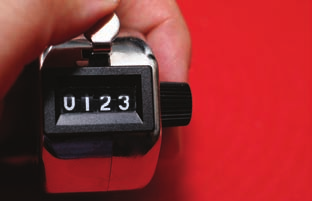
\includegraphics[width=0.4\linewidth]{counter}
		\label{fig:counter}
	\end{figure}
	
	\section*{Exercise 2}
	Implement a class Rectangle. Provide a constructor to construct a rectangle with a
	given width and height, member functions \verb|get_perimeter| and \verb|get_area| that compute
	the perimeter and area, and a member function \verb|void resize(double factor)| that resizes
	the rectangle by multiplying the width and height by the given factor.
	
	\section*{Exercise 3}
	Implement a class \verb|Student|. For the purpose of this exercise, a student has a name and
	a total quiz score. Supply an appropriate constructor and functions \verb|get_name()|,
	\verb|add_quiz(int score)|, \verb|get_total_score()|, and \verb|get_average_score()|. To compute the latter,	you also need to store the \emph{number of quizzes} that the student took.
	
	\section*{Exercise 4}
	Design a class \verb*|Message| that models an e-mail message. A message has a recipient, a
	sender, and a message text. Support the following member functions:
	\begin{itemize}
		\item A constructor that takes the sender and recipient and sets the time stamp to the
		current time
		\item A member function \verb|append| that appends a line of text to the message body
		\item A member function \verb|to_string| that makes the message into one long string like this: \verb|"From: Mohamed Yacine\nTo: Nacer Billal\n ..."|
		\item A member function print that prints the message text. Hint: Use \verb|to_string|.
	\end{itemize}
	Write a program that uses this class to make a message and print it.
	
	\section*{Exercise 5}
	Design a class \verb|Mailbox| that stores e-mail messages, using the \verb|Message| class of Exercise 4. Implement the following member functions:
	\begin{verbatim}
		void Mailbox::add_message(Message m)
		Message Mailbox::get_message(int i) const
		void remove_message(int i)
	\end{verbatim}	
\end{document}